\documentclass[12pt,]{article}
\usepackage{lmodern}
\usepackage{amssymb,amsmath}
\usepackage{ifxetex,ifluatex}
\usepackage{fixltx2e} % provides \textsubscript
\ifnum 0\ifxetex 1\fi\ifluatex 1\fi=0 % if pdftex
  \usepackage[T1]{fontenc}
  \usepackage[utf8]{inputenc}
\else % if luatex or xelatex
  \ifxetex
    \usepackage{mathspec}
    \usepackage{xltxtra,xunicode}
  \else
    \usepackage{fontspec}
  \fi
  \defaultfontfeatures{Mapping=tex-text,Scale=MatchLowercase}
  \newcommand{\euro}{€}
\fi
% use upquote if available, for straight quotes in verbatim environments
\IfFileExists{upquote.sty}{\usepackage{upquote}}{}
% use microtype if available
\IfFileExists{microtype.sty}{%
\usepackage{microtype}
\UseMicrotypeSet[protrusion]{basicmath} % disable protrusion for tt fonts
}{}
\usepackage[margin=1in]{geometry}
\usepackage{graphicx}
\makeatletter
\def\maxwidth{\ifdim\Gin@nat@width>\linewidth\linewidth\else\Gin@nat@width\fi}
\def\maxheight{\ifdim\Gin@nat@height>\textheight\textheight\else\Gin@nat@height\fi}
\makeatother
% Scale images if necessary, so that they will not overflow the page
% margins by default, and it is still possible to overwrite the defaults
% using explicit options in \includegraphics[width, height, ...]{}
\setkeys{Gin}{width=\maxwidth,height=\maxheight,keepaspectratio}
\ifxetex
  \usepackage[setpagesize=false, % page size defined by xetex
              unicode=false, % unicode breaks when used with xetex
              xetex]{hyperref}
\else
  \usepackage[unicode=true]{hyperref}
\fi
\hypersetup{breaklinks=true,
            bookmarks=true,
            pdfauthor={Lisa MALIPHOL},
            pdftitle={Diateam SCAD@COPS A Hybrid Network Intrusion Detection System},
            colorlinks=true,
            citecolor=blue,
            urlcolor=blue,
            linkcolor=magenta,
            pdfborder={0 0 0}}
\urlstyle{same}  % don't use monospace font for urls
\setlength{\parindent}{0pt}
\setlength{\parskip}{6pt plus 2pt minus 1pt}
\setlength{\emergencystretch}{3em}  % prevent overfull lines
\setcounter{secnumdepth}{5}

%%% Use protect on footnotes to avoid problems with footnotes in titles
\let\rmarkdownfootnote\footnote%
\def\footnote{\protect\rmarkdownfootnote}

%%% Change title format to be more compact
\usepackage{titling}

% Create subtitle command for use in maketitle
\newcommand{\subtitle}[1]{
  \posttitle{
    \begin{center}\large#1\end{center}
    }
}

\setlength{\droptitle}{-2em}
  \title{Diateam\\SCAD@COPS\\A Hybrid Network Intrusion Detection System}
  \pretitle{\vspace{\droptitle}\centering\huge}
  \posttitle{\par}
  \author{Lisa MALIPHOL}
  \preauthor{\centering\large\emph}
  \postauthor{\par}
  \date{}
  \predate{}\postdate{}



\begin{document}

\maketitle


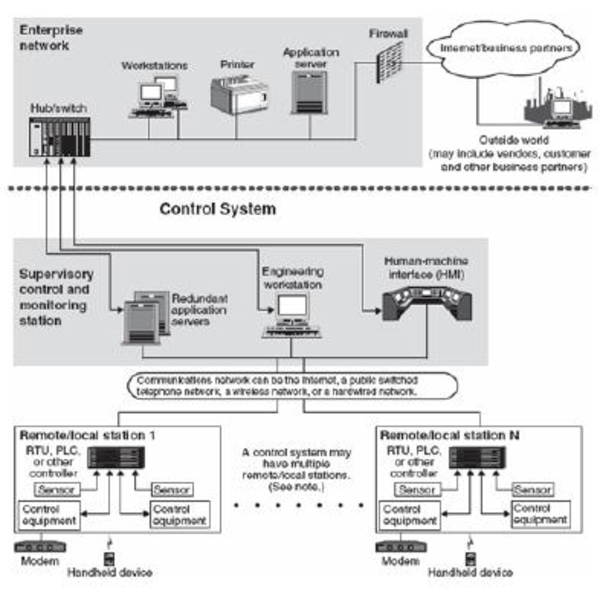
\includegraphics{test2_files/figure-latex/unnamed-chunk-3-1.pdf}

\thispagestyle{empty} \clearpage

\begin{center}

\vspace{30mm}

{\Huge Diateam: SCAD@COPS}\\
\bigskip
{\Huge A Hybrid Network Intrusion Detection System}\\
\vspace{15mm}
{\Large by}\\

\vspace{18mm}
{\huge Lisa MALIPHOL}\\

\vspace{25mm}

\textit{A thesis submitted in partial satisfaction of the}\\
\medskip
\textit{requirements for the diploma of the}\\
\medskip
\textit{Masters of Science}\\
\medskip
\textit{in}\\
\medskip
\textit{Computer Science and Decision Systems}\\
\medskip
\textit{in the}\\
\medskip
\textit{Grande École}\\
\medskip
\textbf{\textit{\Large Télécom Bretagne}}\\

\vspace{10mm}

\textit{Academic Advisors:}\\
\medskip
\textit{Professor Yannis Haralambous}\\
\medskip
\textit{Professor Sandrine Vaton}\\

\vspace{15mm}

\textit{September 2015}\\
\medskip
\textit{Plouzane, FRANCE}\\

\end{center}

\thispagestyle{empty} \clearpage

\tableofcontents

\thispagestyle{empty} \newpage

\section*{Acknowledgements}\label{acknowledgements}
\addcontentsline{toc}{section}{Acknowledgements}

In memory of my late mother, Pisamai Maliphol, if only she could have
witnessed not only her latest grandchild, but to see me make it through
the completion of this masters degree. In many ways, these two years
were part of the healing process after her loss. She would have been
extremely proud.

This work is also dedicated to my children, Mintra, Samya, and Lucien,
may they never cease to continue and to have the motivation and
curiosity to learn, no matter how late in life.

Not enough gratitude can be expressed to Nehme Boghdadi and Aimee
Johansen. You both were there to encourage and to help along the
journey, especially during difficult times. I would not have done this
without you guys.

Thank you to Guillaume Prigent and all the folks at Diateam for
providing a convivial environment in which to work. Not only did I have
much to learn there technically, but lessons in the French language and
culture that I would not have found in the classrooms.

Lastly, I would like to also thank Sandrine Vaton for agreeing to be my
advisor and then encouraging me to take the next step.

\pagebreak

\section*{Abstract}\label{abstract}
\addcontentsline{toc}{section}{Abstract}

\pagebreak

\section{Introduction}\label{introduction}

Supervisory control and data acquisition systems (SCADA) are one type of
industrial control system (ICS) put in place for monitoring and
controlling industrial processes, such as those in the energy or
manufacturing sectors. Originally, these systems were isolated and used
proprietary protocols, whose security relied predominantly on obscurity.
As SCADA systems have moved towards open standards and have become more
interconnected to traditional information technology systems, these
critical systems have also become increasingly exposed and targeted to
cyber attacks.{[}Zhu2010{]}{[}Zhu2011{]}

To secure SCADA systems, intrusion detection systems (IDS) are put into
place with the purpose of observing, analyzing and detecting any
malicious activity, which are then alerted to, and reviewed by, security
analysts. Most IDSs found in the market-place are commonly network,
signature-based IDSs. Anomaly-based detection systems are relatively
immature, however, they provide a greater possibility of detecting
unknown attacks. Signature-based systems can only detect known and
identified signatures of attacks.

The trade-off between the two types of systems, signature-based and
anomaly-based, are predominantly in the the accuracy with which they can
detect a real attack, or anomaly. Although signature-based systems that
have been properly configured rarely raise false alarms, unlike
anomaly-based systems, they are less capable in detecting novel attacks.
Additionally, these intrusion detection systems themselves are also
exposed to the same security issues as the systems they are trying to
secure.

Diateam has proposed an architecture and implemented a prototype of a
hybrid IDS under the project SCAD@COPS. Based on the contributions of
{[}Chifflier2014{]} and {[}Diallo2014{]}, the prototype integrates the
architectural and signature-based aspects as described in their work,
and where the following constraints were taken into consideration in the
design of SCAD@COPS: network-based passive only; the IDS should not
interfere with, nor modify the SCADA system only TCP/IP and Ethernet
data are analyzed.

This work is divided into the following major sections:

\begin{itemize}
\itemsep1pt\parskip0pt\parsep0pt
\item
  Section 2 provides an overview of SCADA systems
\item
  Section 3 provides some basic networking principles
\item
  Section 4 briefly considers a few common cyber attacks
\item
  Section 5 discuss intrusion detection systems
\item
  Section 6 summarizes different approaches for detecting network
  intrusions
\item
  Section 7 lists the tools utilized in this work
\item
  Section 8 describes the data source used in this work
\item
  Section 9 gives an overview of the exploratory data analysis
\item
  Section 10 describes the prototype architecture and implementation
\item
  Section 11 outlines the statistical measures and features used
\item
  Section 12 describes the testing and evaluation process
\item
  Section 13 summarizes and concludes
\end{itemize}

\pagebreak

\section{Overview of SCADA Systems}\label{overview-of-scada-systems}

\subsection{ICS}\label{ics}

An Industrial control system (ICS) comprises such systems as supervisory
controls and data acquisition (SCADA), distributed control systems
(DCS), and smaller systems such as programmable logic controllers (PLC)
that are control systems predominantly used in industrial production.

ICSs were initially developed to meet the requirements of performance,
reliability, safety and flexibility. They existed prior to the
advancement in computer and network technology, such as public and
private networks, desktop computing, or the Internet. Since ICSs
remained rather isolated and obscure, the dangers of cyber security were
less, or non-existent.

Typically industrial control systems are continuously operational and
commonly serve vital public services and infrastructure, thus preventive
security measures must be put into place. The compromise of SCADA
systems may have negative consequences including, but not limited to,
substantial damage to the environment, significant risk to human safety
and health, and financial and production losses.

\subsection{SCADA}\label{scada}

A Supervisory Control and Data Acquisition (SCADA) system is an
industrial control system (ICS) used for monitoring equipment and
controlling processes in industries such as electrical, water, and oil,
as . The administration over a geographically widely distributed process
can be directed from a central location at the master terminal unit
(MTU) in SCADA systems. Changes to process controllers, the opening and
closing of valves and switches, the monitoring and the measurement of
information is administered from the MTU to remote terminal units (RTU).
Due to their economy, versatility, flexibility, and configurability,
programmable logic controllers, which are small industrial computers are
widely used as RTUs.{[}Stouffer2006{]} The various components of a SCADA
system is shown (Figure 1).

These systems have differing constraints and properties from those of
traditional IT systems, the most prominent being that they are hard
real-time systems that must always be available and run continuously
without outage. Once the field devices have been put into place, they
are normally left untouched, i.e., not rebooted and left running for
years. This creates the problem of the systems being more susceptible to
buffer overflow due to the accumulation of fragmentation.{[}Zhu2011{]}

Historically, SCADA systems resided on their own internal networks and
were not connected to other networks. They used proprietary protocols,
and were, therefore, less vulnerable to network attacks. However, over
time as these systems adopted open standards and leveraged traditional
enterprise systems to lower costs, to increase functionality and
productivity, SCADA systems are also now increasingly exposed to
internal and external attacks.

\begin{figure}

{\centering 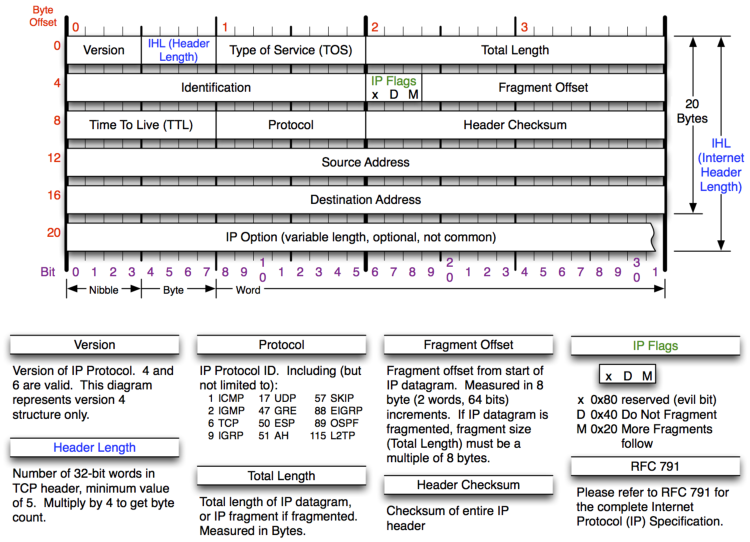
\includegraphics{test2_files/figure-latex/unnamed-chunk-5-1} 

}

\caption{SCADA components [Zhu2010]}\label{fig:unnamed-chunk-5}
\end{figure}

\subsection{Traffic characterization}\label{traffic-characterization}

As seen in the comparative analysis done in {[}Barbosa2012-1{]}, it is
shown how the traffic greatly differs between SCADA and traditional
networks. Most traffic is generated by automated processes in SCADA
networks as opposed to human-generated traffic predominant in
traditional networks. The traffic pattern generated in SCADA networks
have been found to be fairly static and repetitive, with its network
topology unchanging, or rarely modified. Also seen {[}Cheung2006{]} are
a limited number of applications and protocols that run on industrial
systems. Markedly seen over MODBUS traffic, the messages exchanged
between PLCs are recurrent giving it a fixed pattern and relatively
stationary process.{[}Goldenberg2013{]}{[}Barbosa2012-2,3{]}

\pagebreak

\section{Networking Overview}\label{networking-overview}

In this section, a few fundamental networking terms are discussed.
First, an outline of the OSI model is described, followed by the TCP/IP
and MODBUS/TCP protocols.

\subsection{OSI}\label{osi}

Known as the Open System Interconnection (OSI) model, it was initially
developed by the International Standards Organization (ISO) to define
and characterizes the communication between computing systems. The OSI
model, as shown in Figure 2
(\href{https://engineering.linkedin.com/endorsements/geographic-trends-skills-using-linkedins-endorsement-feature}{OSI
Model image source}) is represented as layers, each one expressed as a
protocol. Each layer serves the layer above it, and the lowest one being
closest to the physical medium carrying the communication. Figure OSI
Model depicts each layer and its role and responsibilities.

\begin{figure}

{\centering 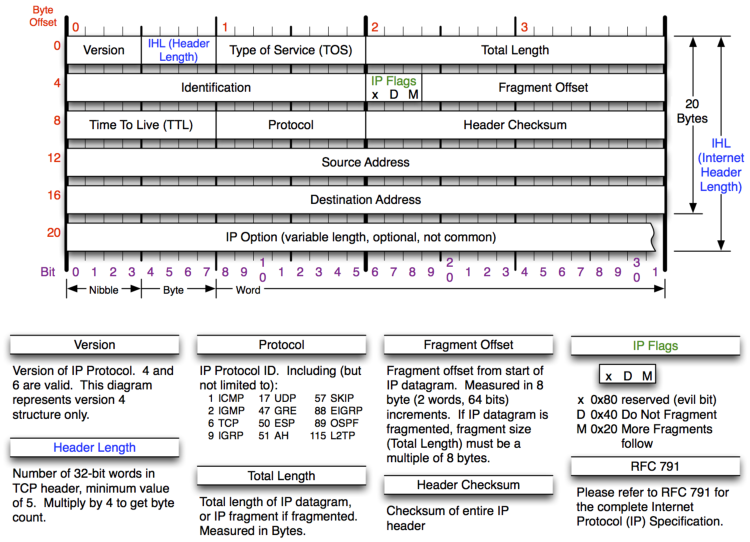
\includegraphics{test2_files/figure-latex/unnamed-chunk-6-1} 

}

\caption{OSI Model}\label{fig:unnamed-chunk-6}
\end{figure}

\subsection{Protocols}\label{protocols}

As SCADA systems have become increasingly interconnected to enterprise
networks, they operate over, and utilize the same protocols as
previously discussed. Additionally, most SCADA appliances implement and
use the MODBUS/TCP protocol, which run over the TCP protocol.

\subsubsection{Transmission Control Protocol/Internet Protocol
(TCP/IP)}\label{transmission-control-protocolinternet-protocol-tcpip}

Initially developed by the Defense Advanced Research Project Agency
(DARPA) in the late 1960s, the Internet protocol suite was the result of
the research and development of data transmission technologies in the
United States that was used as a standard for military computer
networking.

TCP/IP provides reliable, ordered and error-checked delivery of streams
of octets between applications running on hosts communicating over an IP
network. A detailed illustration of the TCP and IP headers can be seen
in Figures 3
(\href{http://nmap.org/book/images/hdr/MJB-TCP-Header}{Image credit: Max
Baxter}) and 4
(\href{http://nmap.org/book/images/hdr/MJB-IP-Header}{Image credit: Max
Baxter}).

\begin{figure}

{\centering 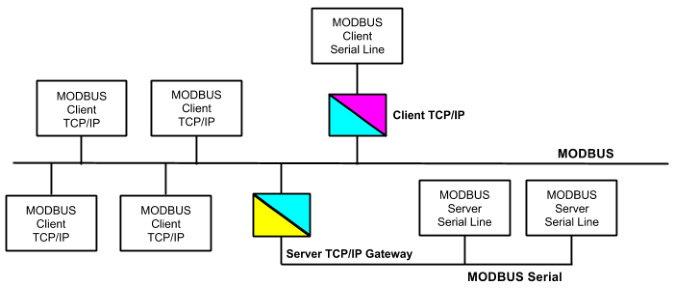
\includegraphics{test2_files/figure-latex/unnamed-chunk-7-1} 

}

\caption{TCP Header}\label{fig:unnamed-chunk-7}
\end{figure}

\begin{figure}

{\centering 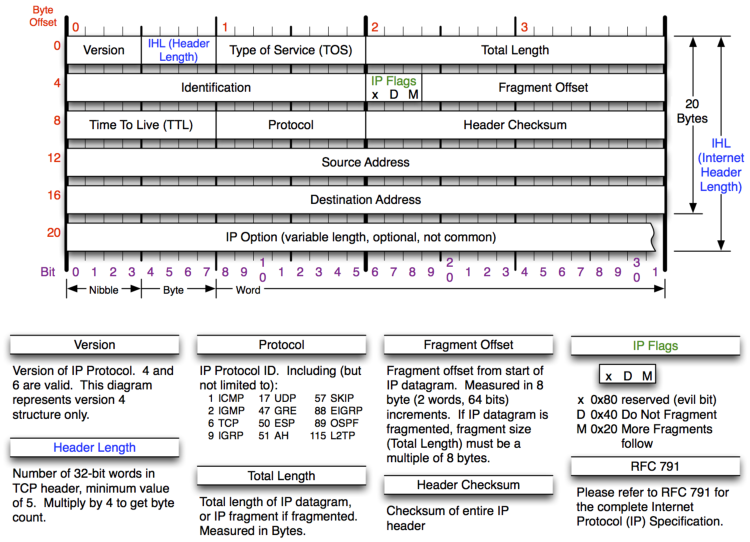
\includegraphics{test2_files/figure-latex/unnamed-chunk-8-1} 

}

\caption{IPv4 Header}\label{fig:unnamed-chunk-8}
\end{figure}

\subsubsection{MODBUS/TCP}\label{modbustcp}

The MODBUS/TCP protocol is an open standard and popular network protocol
used for ICS devices. It is a messaging protocol located at the
application layer that was designed to communicate with PLCs in
industrial systems. However, due to the limited resources the PLCs have,
it was created to be a simple protocol that provides no security against
unauthorized commands or interception of data.{[}Modbus2012{]} Figure 5
gives an example architecture for MODBUS TCP communication.

\begin{figure}

{\centering 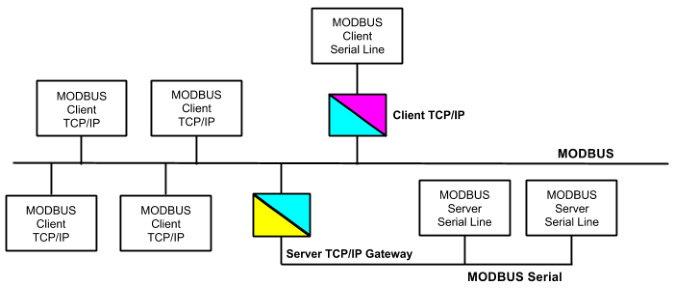
\includegraphics{test2_files/figure-latex/unnamed-chunk-9-1} 

}

\caption{MODBUS TCP/IP Communication Architecture}\label{fig:unnamed-chunk-9}
\end{figure}

The master initiates a request and the slave sends a response containing
either data or error. The common implementations of MODBUS are over
Ethernet networks (MODBUS/TCP) or Serial busses (MODBUS/RTU). Both forms
of MODBUS contain the packet data unit (PDU), the component consisting
of a function code and data.

Attached to the PDU is the application specific addressing and error
checking, which together comprise the application data unit (ADU).
Specific to MODBUS/TCP, the ADU is encapsulated in the TCP packet.
Thereby eliminating the need to include error checking in the MODBUS/TCP
layer, it is left out from the MODBUS/TCP ADU. The MODBUS/TCP frame is
depicted in Figure 6.

\begin{figure}

{\centering 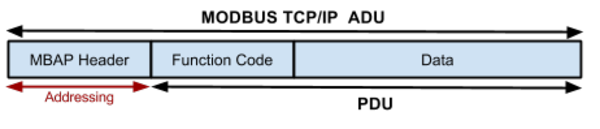
\includegraphics{test2_files/figure-latex/unnamed-chunk-10-1} 

}

\caption{MODBUS/TCP Frame}\label{fig:unnamed-chunk-10}
\end{figure}

Included in the MODBUS Application Protocol (MBAP) are: - Transaction ID
- 2 bytes - identifies request/response pairs - Protocol ID - 2 bytes -
is always 00 00 for Modbus protocol - Length - 2 bytes - identifies the
number of bytes in the following message - Unit ID - 1 byte - used to
distinguish which slave is addressed when several slaves use the same IP
address

The MODBUS/TCP transaction ID is reset to zero with each new TCP
session. It is important to note that in identifying MODBUS
conversations, port 502 is reserved for MODBUS communication. MODBUS
requests are initiated from port 502 and MODBUS responses terminate at
port 502.

As a result of using the simple design of MODBUS and its reliance on the
TCP layer, security issues become apparent. With no authentication and
authorization mechanisms, data integrity checks, or encryption, the
SCADA network components provide no identity or permission verification,
message content legitimacy, or confidentiality.

\pagebreak

\section{Common Attacks on SCADA}\label{common-attacks-on-scada}

\subsection{TShark}\label{tshark}

{[}Hadziosmanovic2010{]}{[}Krotofil2013{]}{[}Lemay2013{]}{[}Rodrigues2011{]}{[}Stouffer2006{]}
define threats and vulnerabilities, security issues, as well as policies
and best practices, and recommendations on how to best secure SCADA
systems. However, cyber attacks continue to increase as SCADA systems
become more exposed and as the attacks grow in sophistication. And
specifically in regards to attacks on MODBUS TCP, little has been
published, except for the work done by Digital Bond.{[}\^{}1{]}
{[}\^{}1{]}: \url{http://digitalbond.com}

Leveraging existing enterprise network infrastructure, SCADA systems are
also at risk to the same threats that typical IT systems encounter. In
addition, as SCADA systems are upgraded less frequently and continue to
run on legacy systems, they are rendered even more vulnerable to various
attacks that may be prevented by deploying upgrades that address newer
and known threats. In {[}Zhu2011{]}, outlines and describes in detail
the various methods of cyber attacks on software and hardware and ways
of compromising SCADA systems.

The following provides an overview of common attacks that have been
exploited against SCADA systems {[}Morris2013{]}.

\subsection{Command Injection}\label{command-injection}

In regards to command injection attacks, the attacker may intercept and
alter, or insert conceivably malicious commands that are then
unknowingly executed in the system. Some known types of command
injection attacks are SQL Injection and Cross-Site Scripting (XSS).
False commands meant to alter the control and configuration in ICSs
commonly seen are injected to modify and interrupt communication and
processes.

More frequently seen in SCADA systems, MODBUS communication is
intercepted, or more precisely, an attacker injects MODBUS functions
intended to modify the industrial process.Since the MODBUS/TCP protocol
was not designed with security taken into account and has no encryption
or sophisticated security precautions, it is vulnerable to the
manipulation of the function code or data field sent in the requests.

\subsection{Response Injection}\label{response-injection}

The nature of response injection attacks is that they perform
unauthorized write requests. Commonly used in ICSs, polling is
continuously done in order to audit the state of remote processes. Over
the MODBUS/TCP, there is frequent request and response communication
between the MTU and RTUs. Perpetrators may craft response packets that
are subsequently inserted into the communication loop and if timed
accordingly, is received as the first response to a query thereby
rejecting further responses as invalid.

\subsection{Denial of Service}\label{denial-of-service}

In an attempt to render services unavailable and stop the proper
functioning of a system, denial-of-service attacks either try to bring
down and crash the service, or flood all resources preventing legitimate
users from accessing the service. Attacks of this type on SCADA systems
try to either reboot MODBUS servers or manipulate the controls to take
them out of service. In other cases, an endpoint is overwhelmed to the
point where it cannot take on further requests.

\subsection{Reconnaissance}\label{reconnaissance}

In a reconnaissance attack there is unauthorized reading of data, where
this type of attack generally surveys a network and identifies connected
devices in order to ascertain the network architecture and topology.
Once the network is accessed by the perpetrator, they may carry out
different levels of scanning over the network, such as address, port and
points scanning. In the case of SCADA systems, with the MODBUS/TCP being
the prevailing protocol used for ICS devices, function scanning is also
done.

\subsection{Zero-day Attacks}\label{zero-day-attacks}

Attacks that exploit previously unknown vulnerabilities and security
holes before a vendor can react and correct them via a patch are known
as zero-day attacks. As deploying upgrades and patches to ICSs are
relatively slow and infrequent, ICSs are highly susceptible to the
weakness discovered in software or hardware before they are corrected. A
well-known malware meant to target industrial PLCs, Stuxnet was designed
to exploit an assortment of zero-day flaws.{[}Karnouskos2011{]}

\pagebreak

\section{Tools}\label{tools}

\subsection[Wireshark - Network Traffic Analysis
Tool]{Wireshark\footnote{\url{https://www.wireshark.org/docs/wsug_html_chunked}}
- Network Traffic Analysis
Tool}\label{wireshark2---network-traffic-analysis-tool}

Developed in 1997 by Gerald Combs originally named Ethereal, Wireshark
is now an Open Source GNU project. It is a network packet analyzer, or
``packet sniffer'', that captures and displays network packets.

Captured network packets are saved in the pcap file format and can be
dissected and parsed by Wireshark in order to analyze its contents. An
important aspect of Wireshark is that of its passive/monitoring nature
and so does not send, manipulate, or modify the data passing over the
network.

An initial packet capture file was created over simulated network
traffic using Wireshark. Using its export facilities, various files were
created for further analysis, with information such as TCP endpoints,
conversations, etc.

\subsection[TShark]{TShark\footnote{\url{https://www.wireshark.org/docs/man-pages/tshark.html}}}\label{tshark3}

Another tool from the Wireshark suite is the command-line tool similar
to tcpdump is tshark, a network protocol analyzer. In addition to
capturing packet data over a live network, it is also capable of
analyzing packets from an existing capture file. TShark was used to
parse out various pertinent variables pertaining to the Modbus/TCP
application protocol enclosed in the packet data.

\subsection{UNIX Utilities}\label{unix-utilities}

In order to further parse and transform the data, the UNIX utility tool
sed, which supports the use of regular expressions, was also used.

\subsection[R - Statistical Tool]{R - Statistical Tool\footnote{\url{http://www.r-project.org/}}}\label{r---statistical-tool4}

R is an Open Source programming language and environment used for
statistical computing and graphics. Initially developed by John Chambers
at Bell Labs as the S language in 1993, R was created as a freely
available version under the GNU project by Ross Ihaka and Robert
Gentleman at the University of Auckland, New Zealand.

Maintained by the R Development Core Team and with an active and growing
community, it provides various statistical and graphical creation
capabilities available under most operating systems, and is extensible
with numerous packages available.

\subsection{C++}\label{c}

\subsection{SQLite3}\label{sqlite3}

\subsection{MongoDB/MySQL}\label{mongodbmysql}

\section*{References}\label{references}
\addcontentsline{toc}{section}{References}

\end{document}
